\chapter{The interactive story}
\label{ch:is}
Most of the research done on narrative generation is contained within the field of Interactive Storytelling (IS). The average observer may not see the difference between a game with a story and a interactive story, and can be forgiven for this is still in open debate within their respective fields. However open the discussion may be there are, albeit subtle, differences. This chapter covers the work done in this field that relates to my own research, and discusses the contrast between the conception of interactive storytelling and video games.

\section{Video Games and Interactive Stories}
The notion that an interactive story is a distinctly different product than video games has been in open discussion ever since video games started having complex stories themselves. In the early years of video gaming (games like \game{Pong}, \game{Pac-Man} and \game{Tetris}) games usually didn't have a story\footnote{That didn't stop people super imposing stories. See: \url{www.smbc-comics.com/?id=2736}}, but then games like \gameby{The Legend of Zelda}{Nintendo R\&D4} became popular that did have a, albeit small, story. At this point in time the distinction between, and especially the semantics, became open for debate.

In this day and age contemporary games often don't get shipped without an attempt at a story, with the exception being \textit{social} games like \gameby{Candy Crush}{King} and \gameby{Bejeweled}{PopCap Games}, the lines between an interactive narrative and video games become blurry. As matter of fact; the term \textit{video games} has recently been under fire. The questions; what makes something a game? What defines a game? The web show \textit{Extra Credits}\footnote{See \url{http://extra-credits.net} episode of 11/27/2013} has a nice answer to this: 
\begin{quote}
[...] We're asked this question all the time, but, you know; I think it's the wrong question. It's a distraction. It does nothing but limits us. It's as if we started to ask: "Well is this really poetry?" when poets moved away from rigid meter or rhyming couplets. [...]
\end{quote}
The fact is, we are in the middle of a semantic war. My opinion is that in another ten years the industry will have a new term to call these works of interactive engagement. As we stand now games put more emphasis on doing and acting within a set of rules; the game mechanics. Whereas interactive stories revolve around the activity of acting out a story without the constriction of mechanics, usually because the only controls a user has are movement controls supplemented with a contextual button to interact with the environment.
 
\section{IS}
The early attempts to understand interactive storytelling came in the form of \game{Tale-Spin}\cite{Meehan77talespin}. Tale-Spin generated textual stories from data that a user created like; scenery, characters, and the problems that needed to be solved. Other work includes the \textit{Oz Projects}\cite{Mateas97anozcentric} that used intelligent agent technology to tackle the challenges in interactive storytelling. In 2006 came the award winning \gameby{Façade}{Michael Mateas and Andrew Stern}\citep{Mateas03facade:an}. This interactive story focusses on the player who is a close friend of two AI characters. During a cocktail party at the AI characters' home the player can support the characters or try to drive a wedge between them. We can't mention interactive storytelling without mentioning former game designer Chris Crawford, who left the world of video games to work on IS. He wrote \textit{Chris Crawford on Interactive Storytelling}\cite{crawford2012chris} which is a deconstruction of the entire field and compares that with traditional video games. 


\section{Dynamic plot generation}
One of the most cited works when dealing with generating plots for interactive systems is Sgouros' 1999 paper \textit{Dynamic generation, management and resolution of interactive plots}\cite{Sgouros199929}. The system proposed in this document dynamically moves the plot forward with the relations and interactions between actors serving as input. Figure~\ref{fig:sgouros_flowchart} shows us the flow of Sgouros' \textit{Plot Manager}; the central piece of his interactive story system. Sgouros shows us how we can abstract concepts like relations and events both causal and temporal and defines a syntax used to describe actions actors can make and goals they might have. His system generates so-called Aristotelian plots, where a conflict between antagonistic forces develops out of the initial situation. The plot will move through a sequence of conflicts and always terminates in a unambiguous solution. 

\section{Character-based storytelling}
At the turn of the century we saw a shift from general story generation towards a more character driven approach.
Researchers like Riedl and Mark\cite{Riedl03character-focusednarrative}\cite{riedl2010narrative} and Marc Cavazza\cite{Cavazza:2002:CIS:630325.630747} wanted to make characters within the story context be more outspoken and distinct and worked towards systems that made this possible.
Most of my work has been based on and influenced by Mark Riedl and Michael Young who contributed to the computational planning of a story.
With their papers\cite{Riedl03character-focusednarrative}\cite{Riedl:2003:MIU:860575.860694}\citep{Riedl:2004:IPM:1018409.1018753} they tackle a multitude of challenges from story planners that use character intent to dealing with interactions between users and agents.
They co-authored the IS system \textit{Mimesis}\citep{young2003towards}, that allows storytellers to use a author-centric approach to generating different stories.
My own planning system (further discussed in chapter~\ref{ch:planning}) has taken a similar route as the systems proposed by Riedl and Young.

\section{Generative narrative within games}
I stated at the beginning of this chapter that most research on the subject of narrative generation takes place within the field of interactive storytelling, but there are some commercial games that have used a form of generative narration.
In \gameby{The Elder Scrolls V: Skyrim}{Bethesda Game Studios} the developers implemented a system they called \textit{Radiant A.I.} that tries to dynamically react to the player's actions.
For example, players with a high \textit{Pickpocket} skill would get told to "keep their hands to themselves" by guards.
The \textit{Radiant Quest} system expands on this, giving players quests that suit their skills and send them to places previously unvisited.
This context is usually used within games; representing a 'fixed' story, but with subtle variance that lets each player have their own experience within a game world.


\section{Conclusions}
The related work done within this field is vast.
So vast perhaps, that to dissect it all greatly exceeds the scope wherein this thesis operates.
But most of the research has been focussed on generating a narrative that is "fixed" from the beginning with some leeway towards actual context.
The usage of a narrative planner is almost universal to ensure any kind of plot coherence, as is a form of author input to control the flow of a story.
These basic elements create a interactive story system that can deliver powerful narratives with believable characters.
My own concern is the involvement of the player.
In most examples the player is merely an actor with a more volatile behaviour, instead of his own character.
I strive for a system that really revolves around the player.
The story made by the actions that the player did or did not do.

\begin{figure}[p]
	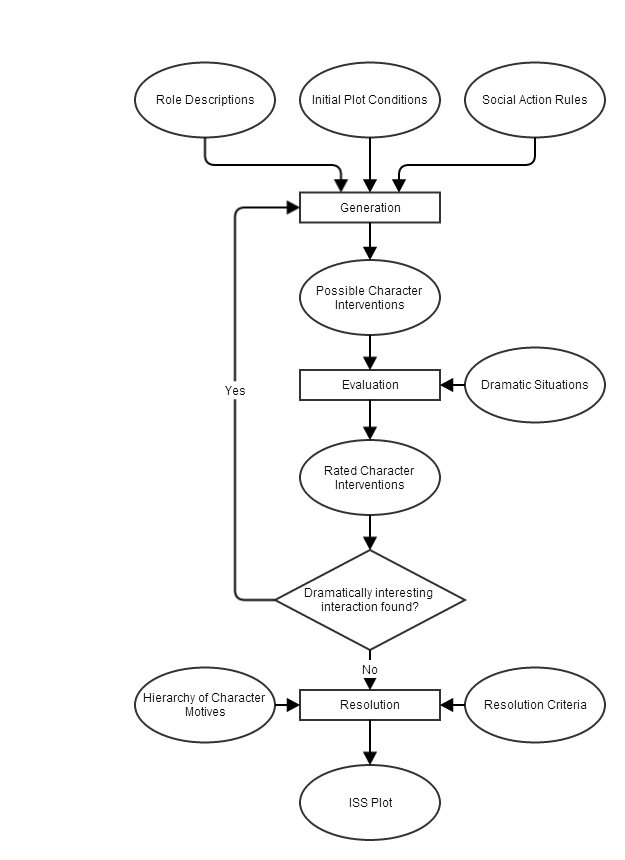
\includegraphics[scale=.6]{sgourosflowchart}
	\caption{Flowchart of Sgouros' \textit{Plot Manager}}
	\label{fig:sgouros_flowchart}
\end{figure}



